\documentclass{article}
\usepackage[utf8]{inputenc}
\usepackage{amsmath}
\usepackage{amssymb}
\usepackage{graphicx}

\title{SHAP-based Average Treatment Effect Calculations}
\author{Kalka, Iris
        \and
        Yacovzada, Nancy}
        
\date{March 2019}

\begin{document}

\maketitle

\section{Introduction}
Causal inference from observational data is a crucial an challenging field of work. Often works rely on assessing potential outcomes in order to estimate treatment effects \cite{neyman1923application}\cite{rubin1974estimating}. Many techniques, such as propensity score (PS) techniques, as formalized by Rosenbaum and Rubin \cite{rosenbaum1983central}, model observed data in order to predict treatment effects. These techniques enable controlling confounding in non-experimental studies in medicine and epidemiology. 

%TODO: ref 1, is that really what Iris meant to cite? "neyman1923application"

A central issue researchers are facing using such methods is how to select the set of variables to be included in the model estimating for treatment effect. The bias and variance of the estimated treatment effect can depend strongly on which of these candidate variables are included in the PS model \cite{brookhart2006variable}.

One assumption in the potential outcomes framework is ignorability, meaning that there are no unmeasured confounders \cite{rosenbaum1983central}. More specifically, the assumption of ignorability demands that potential outcomes are independent of treatment assignment, conditioned on the set of observed covariates.

A possible limitation of PS methods, as described by Rubin in \cite{rubin1997estimating}, is that a covariate related to treatment assignment but unrelated to the outcome is handled the same as a covariate related to treatment but also strongly related to outcome. Such inclusion of irrelevant covariates might reduce the efficiency of an estimated treatment effect \cite{10.1093/biomet/asx009}. In some cases, the use of pretreatment covariates might even increase bias of treatment effect estimators.

Our work is based on an assumption that every covariate can be treated as a covariate effecting both the treatment and the outcome. 
%TODO: REFINE
We believe that the size of the effect can be computed and taken into account such that pretreatment covariates are nearly ignored whereas other treatments are taken into account. 


\section{Methods}
We compare treatment effect evaluation using several methods. We separate the methods to baseline methods already available in the literature: methods based on an estimator predicting the treatment; methods based on an estimator predicting the outcome; and methods based on two estimators one predicting treatment and the other predicting outcome.

We compare methods by looking at the predicted Average Treatement Effect on Treated (ATT) compared with the true known ATT. Let us recall the definition of ATT:
\begin{equation*}
    ATT = \mathbb{E}[]Y_1 - Y_0 | T=1]
\end{equation*}

For all of these evaluations we used the Scikit-Learn gradient boosting predictors with default parameters \cite{scikit-learn}. 

\subsection{Baseline}
Our first method of estimating ATT is Inverse Propensity Score Weighting (IPW).
We use the following equation for calculation of ATT:
\begin{equation*}
    \begin{split}
        ATT = & \mathbb{E}[Y_1 - Y_0 | T=1] \\
        = & \mathbb{E}_X[\mathbb{E}[Y_1 - Y_0 | X, T=1]] \\
        = & \mathbb{E}_X[\mathbb{E}[Y_1 | X, T=1] - \mathbb{E}[Y_0 | X, T=1]]
    \end{split}
\end{equation*}

Under strongly ignorable treatment assumption the potential outcomes $Y_0$, $Y_1$ are independent of the treatment selection given the observed covariates $X$. Therefore:
\begin{equation*}
    ATT = \mathbb{E}_X[\mathbb{E}[Y_1|X, T=1] - \mathbb{E}[Y_0 | X, T=0]]
\end{equation*}

Thus we use the propensity score and the inverse probability of treatment weighting to compute ATT \cite{abdia2017propensity}. 

The two other methods of baseline estimation relay on matching functions. For every treated individual we locate the most similar untreated individual. Thus estimating the treatment effect for every treated individual. This method uses the Scikit-learn Nearest neighbors tool for identification of the most similar individual \cite{scikit-learn}. 

Given a distance matrix between all individuals ATT is computed through matching by calculating the average difference in outcome for every treated individual. This is done by the difference between the individual's true outcome and the mean outcome of $k$ nearest untreated neighbors based on the given distance matrix. The total ATT is then the average of all treated individuals' average difference in outcome.

Distance (and inversely similarity) between individuals is computed based solely on the propensity score computed for each individual. The two methods of distance used by us are Euclidean distance and Mahalanobis distance.


\subsection{Based on treatment prediction}
When accounting for the difference in effects of each covariate we chose to look at the feature importances in the treatment predictor. In order to make the different features importances comparable we use SHapley Additive exPlanations (SHAP) values \cite{lundberg2017unified}. These values are scalar values explaining the individual contribution of each covariate for each individual in the estimation of the treatment. 

Given a matrix of $N\times{}M$ covariates (where $N$ is the number of individuals and $M$ is the number of covariates) we create a single predictor $\mathcal{M}$ from the covariates to the treatment (marked a as a binary value). We then compute the SHAP values of $\mathcal{M}$ for every individual resulting in an $N\times{}M$ matrix. 

Our distances are computed based on the SHAp values matrix using either Euclidean of Mahalanobis distance for every two individuals. Afterwards the ATT is calculated using matching. 

\subsection{Based on outcome prediction}
We create a single predictor that predicts the outcome given both an $N\times{}M$ matrix of covariates and a boolean vector of length $N$ of the treatment. After prediction of outcome we compute the SHAP values of all input values, giving us a matrix of size $N\times{}(M+1)$. 

Our computed distance should be reflective only on pretreatment features. It should not account for whether an individual is treated or not. Therefore, we remove the SHAP value respective of the treatment assignment, yielding us a matrix of $N\times{}M$. 

The given matrix is then used to compute distances either through Euclidean distance of Mahalanobis distance between every two individuals. ATT is then calculated using matching based on the distance measures. 

\subsection{Based on treatment prediction and outcome prediction}
We create two predictors. One predictor $\mathcal{M}_T$ predicts the treatment assignment from covariates.The second predictor $mathcal{M}_Y$ predicts the outcome from both the covariates and the treatment assignment. 

We compute the SHAP values from both treatment and outcome predictions ($S_T$ and $S_Y$ respectively). In order to have comparable SHAP values we remove the column related to treatment from the $S_Y$ matrix. 

At this point each individual is represented with two vectors of length $M$ (number of covariates). We then join the vectors by dividing the values in $S_Y$ by those in $S_T$ in an element-wise division. Thus each person is represented with a single combined vector of length $M$.

Distances between individuals are computed using either Euclidean or Mahalanobis distances on combined vectors. ATT is computed using matching based on the distance matrix.

\subsection{Simulation}
\subsubsection{Kang-Schafer}
Our first method of simulation is the Kang-Schafer method for creating simulated data \cite{kang2007demystifying}. This method assigns four random covariates for every individual ($x_i^j~\mathcal{N}(0,1)$ for every $i\in{}\{1,2,3,4\}$). 
Propensity is then computed in the following way:
\begin{equation*}
    p(T=1| X=x) = \frac{1}{1 + \exp{(x_1 - \frac{x_2}{2} + \frac{x_3}{4} + \frac{x_4}{10})}}
\end{equation*}

We then assign treatment using the true propensity score as the probability for a binomial variable, yielding treatment assignments that are binary. 

Given both the covariates and the treatment assignments, we compute a expected outcome as:
\begin{equation*}
    \mathbb{E}[Y|X=x, T=t] = 210 + t + 27.4 \cdot{} x_1 + 13.78 \cdot{} x_2 + 13.7 \cdot{} x_3 + 13.7 \cdot{} x_4
\end{equation*}

Under the strong ignorability assumption and equations from the Kang-Schafer paper we can compute the true ATT using the following steps:
\begin{equation*}
    \begin{split}
        ATT = & \mathbb{E}[Y_1 | X=x, T=1] - \mathbb{E}[Y_0 | X=x, T=1] \\
        \mathbb{E}[Y_1|T=1, X=x] = & \mathbb{E}[Y|T=1, X=x] \\
        \mathbb{E}[Y_0|T=1, X=x] = & \mathbb{E}[Y_0|T=0, X=x] = \mathbb{E}[Y|T=0, X=x] \\
    \end{split}
\end{equation*}
Therefore $ATT=\mu{}^{(1)} - \mu{}^{(0)} = 200-220 = -20$ 
%TODO: is this actually -20?

\subsubsection{Z-Bias}
Our second method of simulation is based on adjusting for instrumental biases. We implemented two types of simulations according to the Z-Bias generation process as described in Myers \textit{et al} \cite{myers2011effects}.

The simulation creates examples where there are: one instrumental variable $Z$, one unobserved variable affecting both treatment and outcome $U$, a treatment $X$ and an outcome $Y$. All four variables are binary. These are all described in Figure \ref{fig:z_bias_explanation} from the original paper.

\begin{figure}
    \centering
    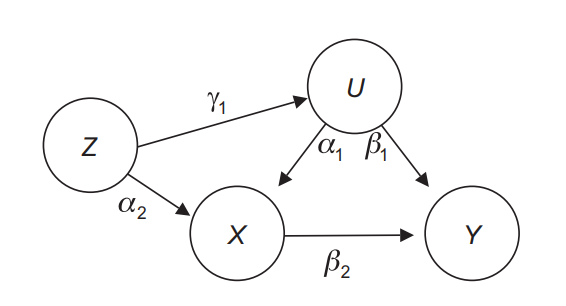
\includegraphics[width=\textwidth]{Paper/images/z_bias_schema_complex.png}
    \caption{A figure from Myers \textit{et al} depicting the relationships between variables in simulated data.}
    \label{fig:z_bias_explanation}
\end{figure} 

There are two methods of simulation we use, an additive and a multiplicative version. In both versions the order of variables simulated is consistent in order to ensure that the risk of outcome would depend directly on $U$ and $X$ and indirectly on $Z$.

In the additive version of the simulation the first variable to be simulated is $Z$ that is created with the probability $P(Z=1)=0.5$.
Next the unobserved variable is simulated so that $P(U=1|Z)=\gamma{}_0 + \gamma{}_1\cdot{}Z$. Next the treatment is simulation using $P(X=1|U,Z) = \alpha{}_0 + \alpha{}_1 \cdot{} U + \alpha{}_2 \cdot{} Z$. Last we simulate the outcome using $P(Y=1|X,U) = \beta{}_0 + \beta{}_1 \cdot{} U + \beta{}_2 \cdot{} U$.

In the multiplicative version of the simulation the order of simulation is identical to that in the additive version. Probabilities are computed in a different format as is explained in the following equations:
$$P(Z=1)=0.5$$
$$P(U=1|Z)=\gamma_0\cdot{}(\gamma_1^Z)$$
$$P(X=1|U,Z)= \alpha_0\cdot(\alpha_1^U)\cdot(\alpha_2^Z)$$
$$P(Y=1|X,U) = \beta_0 \cdot (\beta_1^U) \cdot (\beta_2^X)$$

\subsection{Results}
% TODO: Consider adding the figure of Y and T shap values in the Kang-Schafer simulation. This needs to be recreated using the current simulation but is still doable. 


We simulated a data of $10,000$ individuals using the Kang-Schafer method explained above. We then use the aforementioned methods to estimate the ATT. For each method we estimated the ATT values using matching on $k$ neighbors, where $k=1,2,...,30$. Results of depicted in Figure \ref{fig:kang_schafer}.

\begin{figure}
    \centering
    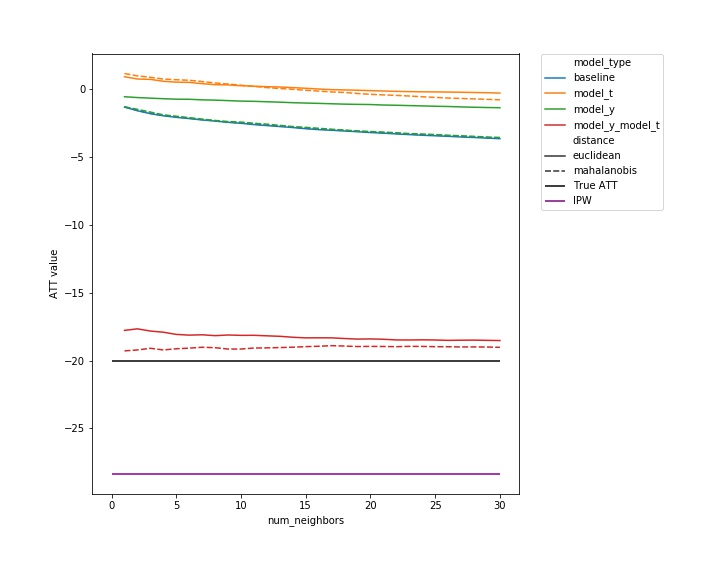
\includegraphics[width=\textwidth]{Paper/images/kang_schafer_ATE_estimations_by_neighbor.jpg}
    \caption{\textbf{ATT Estimations for Kang-Schafer Simulation}: This image shows estimated values of ATT on the Kang-Schafer simulated data. True ATT value is $-20$ and is show in a black solid line. The inverse propensity weighing is marked in a purple solid line. The rest of the estimators are drawn in style according to the distance function used for nearest neighbor matches - Euclidean or Mahalanobis. Color of estimations are saperated by the values used in distance measurements of samples: baseline, based on treatment predicting model, based on outcome predicting model, based on the combination of outcome and treatment prediction models. The $x$ axis is the number of neighbors considered in the nearest neighbor algorithm.}
    \label{fig:kang_schafer}
\end{figure}

We can see that IPW estimation gives an opposite direction of error in estimation compared to all other ATT estimation methods. In edition we can see that ATT estimations based solely on SHAP values from the model predicting treatment yielded the worst results. Following are baseline models and models based solely on the SHAP values from the model prediction the outecome. The best results we given with using SHAP values combination from a model predicting the treatment and a model predicting the outcome. 

For all models it is shown that both the Euclidean and the Mahalanobis distance functions yielded similar results, thus showing a minimal effect. 

In addition we can see that although there is some effect on the number of neighbors considered during matching, this effect occurs mostly for very small number of neighbors and is vastly smaller when taking into account more than five neighbors. 

\textbf{TODO: Add Z bias results here. }

\section{Discussion}
In the framework of potential outcomes an assumption of ignorability is usually made. This assumption relies on independence between treatment and outcome given covariates. However, reality shows that not all covariates should be considered, as some are in fact instrumental variables effecting only the treatment assignment directly. 

Our work aims to create a framework allowing consideration of all covariates while accounting for a difference in effect on treatment and outcome. 

Our results show the the shared consideration of both a model predicting the treatment and a model predicting the outcome can indeed overcome issues of instrumental variables. This added value is shown only be relevant when considering both model, where using each model independently has comparable results to baseline estimators.

In addition our work shows little to no impact of the chosen distance function in case of matching when comparing Euclidean and Mahalanobis distances. We remain confident however that matching function based on domain knowledge will give a better estimation of treatment effects. 

\section{Future Work}
The ease of use in our work is meant for cases of high-dimensional data as well as simple data. We believe that the framework created will work well on data with many covariates, however have yet to test it.

Another type of data the framework should be tested on is data with more complex connections. Our current simulations are all based on rather simple relations between variables. A comparison to cases where there are covariate effecting treatment and/or outcome indirectly could give a better understanding of the framework's abilities. This is especially true since the entire framework can also be used on more complex predictors.

Our current framework has only one method of combining the SHAP values of a treatment predicting model and an outcome predicting model. The rational behind using the ratio of SHAP values between the two models is to reduce the impact of covariates that effect the treatment assignment but not the outcome. Although fitting said goal, we hope to try additional methods of combining SHAP values. Specifically we considered using a logarithm of the ration, a ratio of logarithms, an additive factor of the values, etc. 

Another field we have yet to explore is the use of the SHAP values in order to perform feature selection on the data. Cases where there are many covariates can at times result in over-fitted models and thus biased predictions of treatment effect. We hope that accounting for the shared effect of a covariate both on the treatment and the outcome could allow to remove uneccessary covariates in a through a causal look. 

\section{References}

\bibliographystyle{unsrt}
\bibliography{references.bib}

\end{document}Y1Y1